\documentclass{amsart}
\usepackage{amssymb,latexsym}
\usepackage{graphicx}
\usepackage{color}
 \definecolor{MyDarkBlue}{rgb}{0,0.08,0.45}\definecolor{yellow}{rgb}{0.99,0.99,0.70}\definecolor{white}{rgb}{1.0,1.0,1.0}\definecolor{black}{rgb}{0.00,0.00,0.00}
 %\pagecolor{yellow}

\theoremstyle{plain}
\newtheorem{theorem}{Theorem}
\newtheorem{corollary}{Corollary}
\newtheorem*{main}{Main~Theorem}
\newtheorem{lemma}{Lemma}
\newtheorem{proposition}{Proposition}
\theoremstyle{definition}
\newtheorem{definition}{Definition}
\newtheorem{example}{Example}
\theoremstyle{remark}
\newtheorem*{remark}{Remark}
\newtheorem*{notation}{Notation}
\newtheorem*{proofofnullstellensatz}{Proof of Nullstellensatz}
\newtheorem*{proofofproductsofaffinevarieties}{Proof of Theorem \ref{15}}
\numberwithin{equation}{section}
\begin{document}
\title[Complete-simple distributive lattices]
{Algebraic Geometry - Lothar G\"{o}ttsche \\
	Lecture 12}
\author{Wang Yunlei}
%\address{Harbin Institute of Technology\\
%	Harbin}
\email{wcghdpwyl@126.com}
%\urladdr{http://math.uwinnebago.edu/menuhin/}
%\thanks{Research supported by the NSF under grant number
%	23466.}
%\keywords{Complete lattice, distributive lattice,
%	complete congruence, congruence lattice}
%\subjclass[2010]{Primary: 06B10; Secondary: 06D05}
\date{June 19, 2017}
 
\maketitle

\begin{lemma}
	Let $ X,Y $ be varieties and $ Y $ be affine, let $ \varphi:X\to Y $ is a morphism. Then $ \varphi(X) $ is dense in $ Y $ if and only if $ \varphi^\ast $ is injective.
\end{lemma}\label{21}
\begin{proof}
	If $ \varphi $ is not dense, then there exists a closed subset $ W\subsetneqq Y $ and $ \varphi(X)\subset W $. We can write $ W=Z(f_1,\dots,f_r) $ for $ f_1,\dots,f_r\in A(X)\subset K(X) $. By possibly taking a bigger $ W $ we can write $ W=Z(f) $ for some none zero element $ f\in A(X) $. Now we find $ \varphi^\ast f=f\circ\varphi =0 $, so $ \varphi^\ast $ is not injective. Conversely, if some $ f\neq 0 \in K(X) $ satisfies $ \varphi^\ast f=0 $, then $ \varphi(X)\subset Z(f)\subsetneqq Y $ is not dense.
\end{proof}
\begin{theorem}\label{22}
	Let $ X,Y $ be varieties, there is a bijection
	$$
	\left\lbrace\begin{array}{c}
	\text{dominant rational maps} \\
	\varphi:X \to Y
	\end{array}\right\rbrace\longleftrightarrow\left\lbrace\begin{array}{c}
	k-\text{algebra homomorphisms}\\
	\varphi^\ast:K(Y)\to K(X)
	\end{array}\right\rbrace.
	$$
	In particular, $ X $ and $ Y $ are birational if and only if $ K(Y)\simeq K(X) $.
\end{theorem}
\begin{proof}
	We only need to construct the inverse  map to $ \varphi\to \varphi^\ast $. Let $ \phi:K(Y)\to K(X) $ be a $ k $-algebra homomorphism, we want to construct a rational map $ \varphi:X\to Y $ such that $ \varphi^\ast=\phi $. Replacing $ Y $ by an open affine subset, we can now assume $ Y\subset \mathbb{A}^n $ is closed. Let $ y_1,\dots,y_n\in A(Y) $ be coordinate functions, then $ \phi(y_1),\dots,\phi(y_n)\in K(X) $. We can find a nonempty open subset $ U\subset X $ such that $ \phi(y_i)\in\mathcal{O}_X(U) $ for all $ i=1,\dots,n $. Then the map $ x\to (\phi(y_1)(x),\dots,\phi(y_n)(x)) $ is a morphism from $ U $ to $ Y $. In fact, we restrict $ \phi $ to $ A(Y) $, then $ \phi $ defines an injective homomorphism from $ A(Y) $ to $ \mathcal{O}_X(U) $. Then by theorem \ref{12}, we get a morphism $ \varphi:U\to Y $ and by lemma \ref{21} its image is dense in $ Y $. Thus we find $ \varphi:X\dashrightarrow Y $ which is dominant and $ \varphi^\ast=\phi $.
\end{proof}
\begin{corollary}
	Let $ X,Y $ be varieties, the following statements are equivalent
	\begin{enumerate}
		\item $ X,Y $ are birational;
		\item $ X,Y $ contain open subsets isomorphic to each other;
		\item $ K(X)\simeq K(Y) $ as $ k $-algebras.
	\end{enumerate}
\end{corollary}
\begin{proof}
(1) $ \Rightarrow $ (2): Let $ \varphi:X\dashrightarrow Y  $ be a birational map with inverse $ \psi :Y\dashrightarrow X $. We can check that $ \psi\circ\varphi $ is the identity on $ U= \mathrm{dom}\varphi\cap \varphi^{-1}(\rm{dom}\psi) $ and $ \varphi\circ\psi $ is the identity on $ V= \mathrm{dom}\psi\cap\psi^{-1}(\mathrm{dom}\varphi) $. Thus $ U $ is isomorphic to  $ V $ by restrict $ \varphi $ on $ U $.

(2) $ \Rightarrow $ (3): $ K(X)\simeq K(U) $, $ K(Y)\simeq K(V) $, and we know $ K(U)\simeq K(V) $, thus $ K(X)\simeq K(Y) $.

(3) $ \Rightarrow $ (1): Just the conclusion of theorem \ref{22}.
\end{proof}

\section{Conclusions We Need From Previous Lectures }
 \begin{theorem}\label{12}
 	Let $ X,Y $ be varieties, assume $ Y\subset \mathbb{A}^m $ be a closed affine variety. Then there is a bijection between morphisms $ X\to Y $ and $ k $-algebra homomorphisms $ A(Y)\to \mathcal{O}_X(X) $:
 	$$\begin{array}{ccc}
 	\{ \text{morphisms } X\to Y \} & \xrightarrow{bijection} & \{ \text{homomorphisms }A(Y)\to \mathcal{O}_X(X) \} \\
 	\varphi & \xrightarrow{\qquad\quad} & \varphi^\ast
 	\end{array}$$
 \end{theorem}
 \begin{definition}
 	Take coordinates $ x_1,x_2 $ on $ \mathbb{A}^2 $ and coordinates $ y_0,y_1 $ on $ \mathbb{P}^1 $, the blowup $ \hat{\mathbb{A}^2} $ of $ \mathbb{A}^2 $ at $ 0 $ is $ \hat{\mathbb{A}^2}=Z(x_1y_1-x_2y_0)\subset\mathbb{A}^2\times \mathbb{P}^1 $.
 \end{definition}
 \begin{remark}
 	$ \hat{\mathbb{A}^2} $ is closed in $ \mathbb{A}^2\times\mathbb{P}^1 $. Closed subsets of $ \mathbb{A}^n\times\mathbb{P}^m $ are zero sets $ Z(F_1,\dots,F_r) $ where $ F_i\in k[x_1,\dots,x_n,y_0,\dots,y_m] $ are homogeneous in $ y_i $.
 \end{remark}
 \begin{definition}
 	Let $ \Pi=p_1:\hat{\mathbb{A}^2}\to \mathbb{A}^2 $, $ E:=\Pi^{-1}(0) $ is called the exceptional divisor. 
 \end{definition}
 	We can see that $ \Pi $ is a birational morphism because $ \Pi|_{\hat{\mathbb{A}^2}\backslash E}:\mathbb{A}^2\backslash E\to \mathbb{A}^2\backslash \{ 0 \} $ is an isomorphism. In fact $ E=\{ 0 \}\times \mathbb{P}^1 $. 
 \begin{remark}
 	\begin{enumerate}
 		\item Let $ ((x_1,x_2),[y_0,y_1])\in \hat{\mathbb{A}^2}\backslash E $, assume $ x_1\neq 0 $, then we get $ x_2=\frac{y_1}{y_0}x_1 $. It is equivalent to $ (x_1,x_2)\in [y_0,y_1] $. So $ \hat{\mathbb{A}^2} $ is the graph of the canonical morphism
 		$$
 		\begin{array}{ccc}
 		\mathbb{A}^2\backslash \{0\} & \to & \mathbb{P}^1\\
 		(x_1,x_2) & \to & [x_1,x_2].
 		\end{array}
 		$$
 		\item $ U_{y_0}:=\hat{\mathbb{A}^2}\backslash Z(y_0)=\{((x_1,x_2),[1,u])\in\mathbb{A}^2\times \mathbb{P}^1|x_2=ux_1 \} $ is isomorphic to $ \mathbb{A}^2 $ by the morphism $ ((x_1,x_2),[1,u])\to (x_1,u) $ with inverse $ (x_1,u)\to ((x_1,ux_1),[1,u]) $. In the same way $ U_{y_1}:=\hat{\mathbb{A}^2}\backslash Z(y_1)=\{ ((x_1,x_2),[t,1])\in \mathbb{A}^2\times\mathbb{P}^1|x_1=tx_2 \}$ is isomorphic to $ \mathbb{A}^2 $. Then we get $ \hat{\mathbb{A}^2}=U_{y_0}\cup U_{y_1} $, the union of irreducible open cover, so $ \hat{\mathbb{A}^2} $ itself is also irreducible. 
 	\end{enumerate}
 \end{remark}
 In $ U_{y_0} $ the exceptional divisor $ E $ is $ Z(x_1) $, and in $ U_{y_1} $ the exceptional divisor $ E $ is $ Z(x_2) $.
 \begin{example}
 	What does the blowup do to a curve $ C\subset \mathbb{A}^2 $ through $ 0 $? Let $ C\subset \mathbb{A}^2 $ be a curve, the strict transform of $ C $ is $$
 	 \hat{C}=\text{ closure of } \Pi^{-1}(C\backslash\{ 0 \}) 
 	$$
 	in $ \hat{\mathbb{A}^2} $. For example, let $ C=Z(F) $, where $ F=x_2^2-x_1^2(x_1+1) $. In the chart $ y_1\neq 0 $, i.e. $ U_{y_0} $, we have 
 	$$
 	\Pi^{-1}(C)=Z(x_1^2(u^2-(x_1+1)))=Z(x_1^2)\cup Z(u^2-(x+1))
 	$$
 	(Note that we talk about this in $ U_{y_0} $, so the exact equation is $ \Pi^{-1}(C)= Z(x_1^2(u^2-(x_1+1)))\cap U_{y_0} $. But we ignore it for simplicity).
 	Since $ Z(x_1^2) $ is exactly the exceptional divisor $ E $, we get $ \hat{C}=Z(u^2-(x+1)) $, and it is isomorphic to $ \mathbb{A}^1 $ by mapping $ ((x_1,x_2),[1,u])\to u $. The inverse of the map is $ u\to ((u^2-1,u^3-u),[1,u]) $. We can see $ C $ and $ \hat{C} $ in the real axes condition
 \begin{figure}[htbp]
 	\centering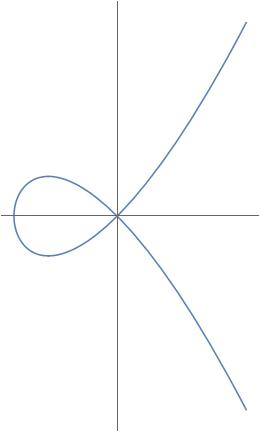
\includegraphics[width=1.4in]{2dimage.jpg}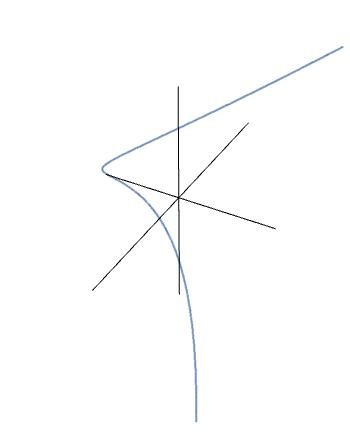
\includegraphics[width=2.0in]{3dimage.jpg}
 	\caption{$ \hat{C}$  in real space }\label{fig:1}
 \end{figure}
 Now we can find that there is no singular point after blowing up.
  \end{example} 
 
% \begin{thebibliography}{9}
 %    \bibitem{a} bibitem
% \end{thebibliography}
\end{document}
